\subsection{Извлечение антропометрических признаков из видео}
Для решения задачи извлечения антропометрических признаков с изображения и видео предложен алгоритм, основанный на  комбинации новейших методов - технике предварительной обработки изображений, алгоритме вычитания фона, алгоритме сегментации изображений на основе разреза графов, алгоритме итеративных ближайших точек.

Процесс извлечения антропометрических признаков объектов на изображении и видео на основе алгоритма компьютерного зрения включает в себя следующие этапы (рис \ref{img14}):
\begin{itemize}
	\item \textbf{Шаг 1:} Предварительная обработка изображения;
	
	\begin{itemize}
		\item Фильтр шума с гауссовым фильтром с матрицей фильтра окна $\left[5 5\right]$;
		\item Используем морфологические операторы - дилатации, чтобы улучшить качество точек изображения со структурами элементов $se=strel\left(line,11,90\right)$;
		\item Эквализация гистограммы.
	\end{itemize}
	\item \textbf{Шаг 2:} Обнаружение объекта и человеческого лица. Важную роль на этом шаге играет алгоритм вычитания фона. Расчетные значения пикселей на разных кадрах получаем по формуле (\ref{eq9});
	
	Метод Виола-Джонса \cite{Violaj2001, Viola2004} используется для обнаружения человеческого лица с изображения. Метод состоит из трех основных этапов: интегральном представлении изображения, метод построения классификатора на основе алгоритма адаптивного бустинга (AdaBoost) и метод комбинирования классификаторов в каскадную структуру.
	\item \textbf{Шаг 3:} Сегментация изображения методом разреза на графах. Поиск области изображения, содержащего части тела человека на основе формулы (\ref{eq25});
	\item \textbf{Шаг 4:} Обнаружение контура и поиск ключевых точек признаков – алгоритм $ICP$. Расчет евклидова расстояния: $d\left(A,B\right) = \sqrt{\left(x_B - x_A\right)^2 + \left(y_B - y_A\right)^2}$;
	\item \textbf{Шаг 5:} Создание антропометрического вектора признаков.
\end{itemize}

\begin{figure}[ht!]
\centering
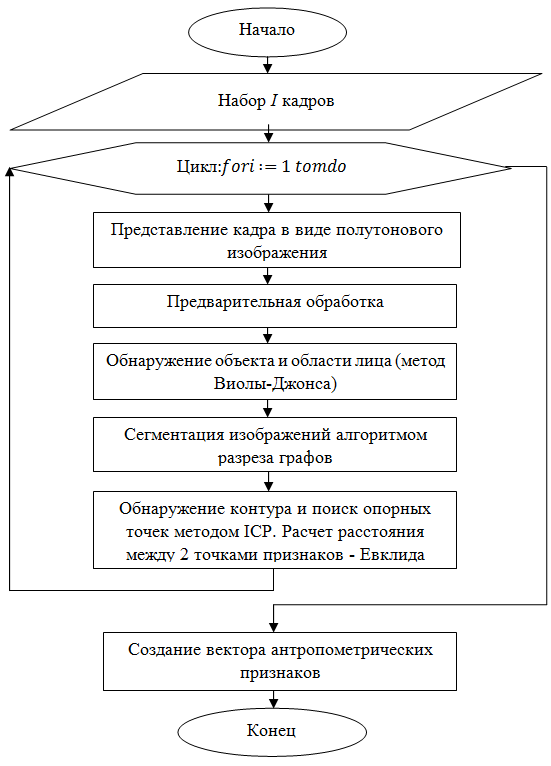
\includegraphics [scale=1.05] {images/h14.png}
\begin{center}
%\captionsetup{justification=justified, labelsep=period}
\caption{Блок-схема алгоритма извлечения антропометрических признаков из видеопоследовательности.} \label{img14}
\end{center}
\end{figure}